\documentclass[../../main]{subfiles}

\begin{document}
\chapter{ヒルベルト空間}
\label{chapter:hilbert_space}
\begin{lead}
\cref{chapter:hilbert_space}で書く予定のことを並べておく.
\end{lead}

\section{無限次元の線型空間}
\subsection{距離空間}

\begin{figure}[htbp]
  \centering
  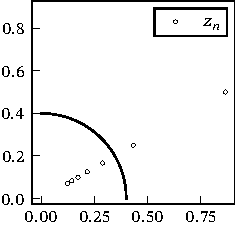
\includegraphics{complex_convergence.pdf}
\end{figure}

\begin{figure}[htbp]
  \centering
  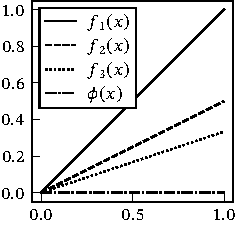
\includegraphics{func_convergence.pdf}
\end{figure}

\subsection{ノルム線型空間}
\subsection{内積空間}
\subsection{ヒルベルト空間}

\section{直交射影}
\subsection{直交射影}

\begin{figure}[htbp]
  \begin{minipage}{\linewidth/2}
    \centering
    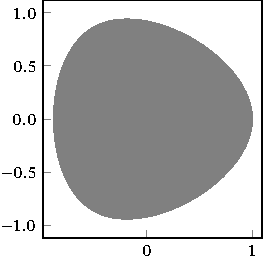
\includegraphics{convex.pdf}
  \end{minipage}%
  \begin{minipage}{\linewidth/2}
    \centering
    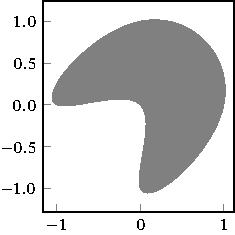
\includegraphics{non_convex.pdf}
  \end{minipage}
\end{figure}

\subsection{直交補空間}
\subsection{正規直交列}

\section{フーリエ級数展開}
\subsection{フーリエ級数展開}
\subsection{フーリエ変換}

\section{多重解像度解析}
\subsection{多重解像度解析}

\begin{figure}[htbp]
  \centering
  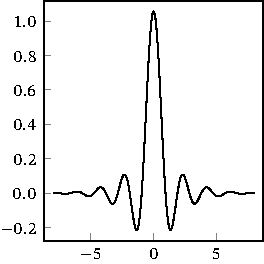
\includegraphics{meyer_scaling.pdf}
\end{figure}

\begin{figure}[htbp]
  \centering
  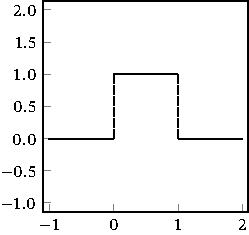
\includegraphics{haar_scaling.pdf}
\end{figure}

\subsection{ウェーブレット変換}

\begin{subappendices}
\section{半ノルムと\texorpdfstring{\(\Lebesgue{p}\)}{Lp}空間}
\end{subappendices}

\section*{演習問題}
\addcontentsline{toc}{section}{演習問題}

\end{document}
